\chapter{Теория}
\label{ch:intro}

\section*{\textbf{LTI системы}}

Система - то, что преобразует сигнал (входной в выходной). \\

Нас не интересует, как работает система, нам интересен только результат, который она дает, поэтому можно представить эту систему
в виде "черного ящика"

\begin{figure}[H]
    \centering
    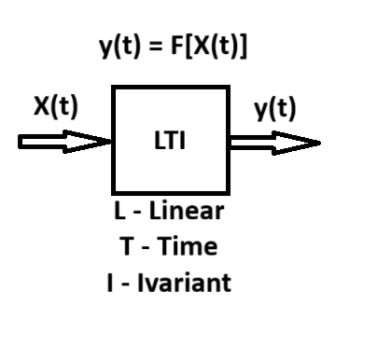
\includegraphics[width=1.0\textwidth]{LTI.png}
    \caption{Визуализация LTI системы}
\end{figure}

Здесь F[x(t)] - функция, выполняемая над входным сигналом x(t), y(t) - результат работы системы (выходной сигнал). \\ 

Примером LTI систем может являться RC цепь

\begin{figure}[H]
    \centering
    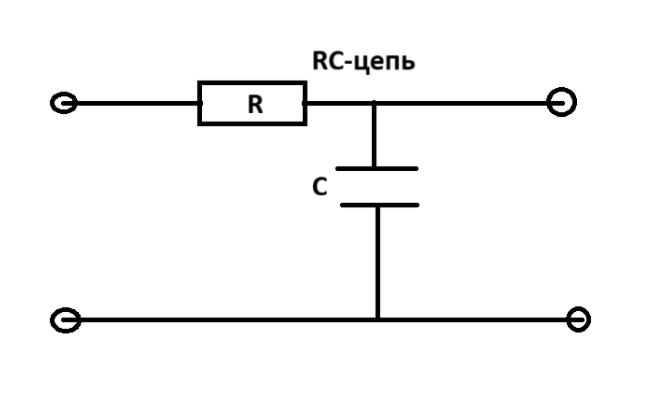
\includegraphics[width=1.0\textwidth]{RC.png}
    \caption{Визуализация RC цепи}
\end{figure}

Подадим на вход такой системы прямоугольный импульс и получим какой-то выходной сигнал:

\begin{figure}[H]
    \centering
    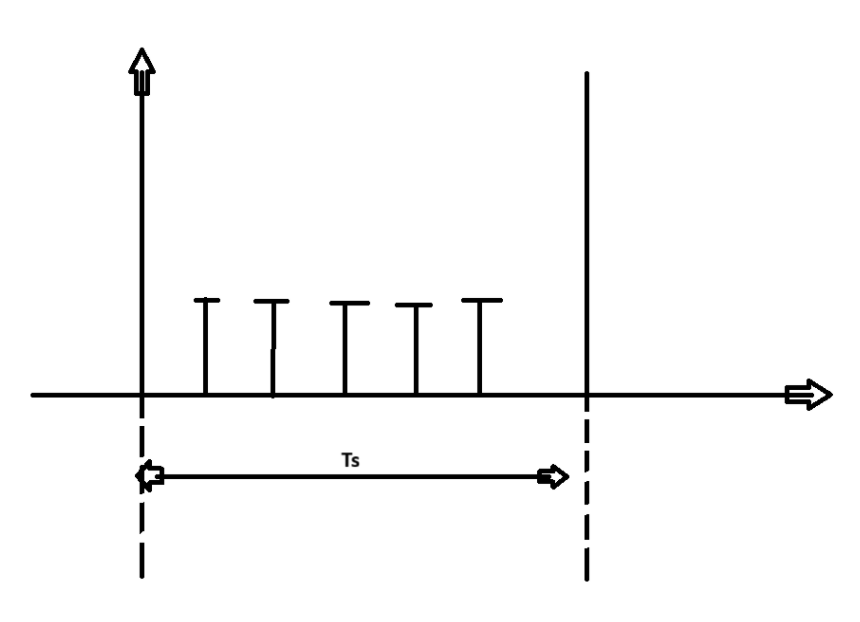
\includegraphics[width=1.0\textwidth]{pulse.png}
    \caption{Визуализация входного и выходного сигнала RC цепи}
\end{figure}

\section*{Линейная, постоянная во времени система. Свойства системы.}

\subsection*{1) Свойство линейности}

Это свойство говорит о том, что реакция на сумму сигналов равна сумме реакций на каждый из сигналов, а также, что при умножении
входного сигнала на какое-то число k получим выходной сигнал, который умножен на k.

\[
x(t) \rightarrow y(t)
\]

\[
K \cdot x(t) \rightarrow K \cdot y(t)
\]

\[
x_1(t) \rightarrow y_1(t) = F[x_1(t)]
\]
\[
x_2(t) \rightarrow y_2(t) = F[x_2(t)]
\]

\[
F[x_1(t) + x_2(t)] = F[x_1(t)] + F[x_2(t)]
\]

\[
s(t) = \sum a_i s_i(t)
\]
\[
y(t) = F\left[\sum a_i s_i(t)\right] = \sum a_i F[s_i(t)]
\]

В линейной системе при подаче линейной комбинации сигналов на входе получают линейную комбинацию выходных сигналов.

\subsection*{2) Свойство постоянства во времени}

Это свойство говорит о том, что если входной сигнал сдвинут во времени на $t_0$, то выходной сигнал тоже будет сдвинут во времени
на $t_0$
\[
y(t) = F[x(t)]
\]
\[
x(t - t_0) \rightarrow y(t - t_0)
\]

\begin{figure}[H]
    \centering
    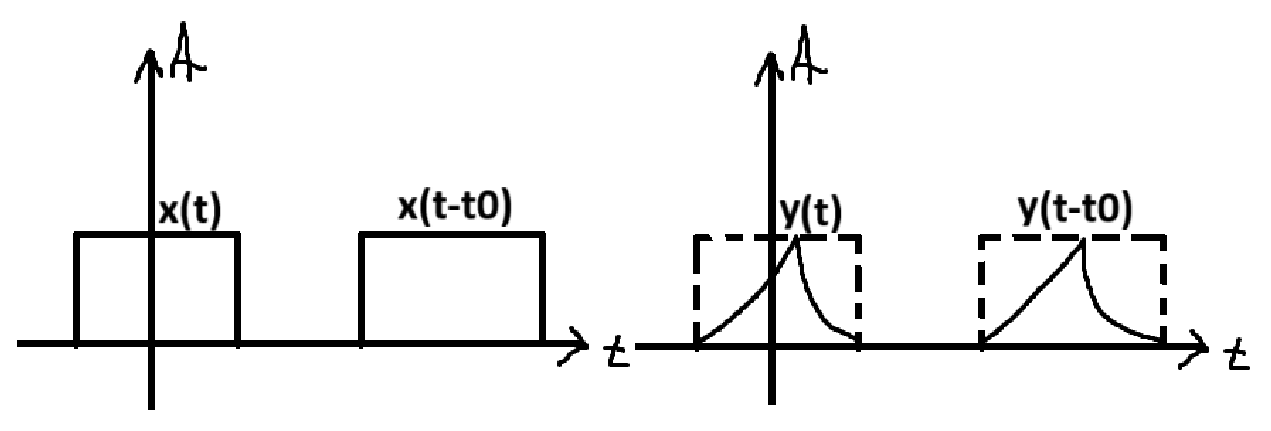
\includegraphics[width=1.0\textwidth]{TI.png}
    \caption{Визуализация свойства постоянства во времени}
\end{figure}

\section*{Реакция системы на произвольный сигнал}

Для определения отклика системы на произвольный входной сигнал нужно выполнить 3 действия:

\begin{enumerate}
    \item Получить реакцию системы на отдельный элементарный сигнал (с небольшой длительностью);
    \item Представить входной сигнал в виде комбинации элементарных сигналов;
    \item Получить выходной сигнал системы при заданном произвольном входном сигнале как сумму реакций на элементарные сигналы.
\end{enumerate}

\section*{Шаг 1}

Выше мы выяснили, как система реагирует на прямоугольный импульс.

\section*{Шаг 2}

Подадим произвольный сигнал на вход системы и аппроксимируем его прямоугольными сигналами (представим входной сигнал в виде комбинации элементарных сигналов).
Пусть прямоугольные сигналы имеют длительность $T_0$, $S$ - произвольная функция, $S_0$ - прямоугольный импульс, $S_0(t)$ - эталонный прямоугольный импульс, тогда
для каждой точки сигнала получим:

\[
s(0) * s_0(t)
\]
\[
s(T_0) * s_0(t - T_0)
\]
\[
s(2T_0) * s_0(t - 2T_0)
\]
\[
s(3T_0) * s_0(t - 3T_0)
\]

В момент времени 0 наша аппроксимирующая функция будет иметь значение $S(0)$ * $S_0(t)$, т.е мы как бы повышаем значение прямоугольного импульса до значения 
входной функции. Далее будем сдвигаться на $T_0$ и повторять процесс.

\begin{figure}[H]
    \centering
    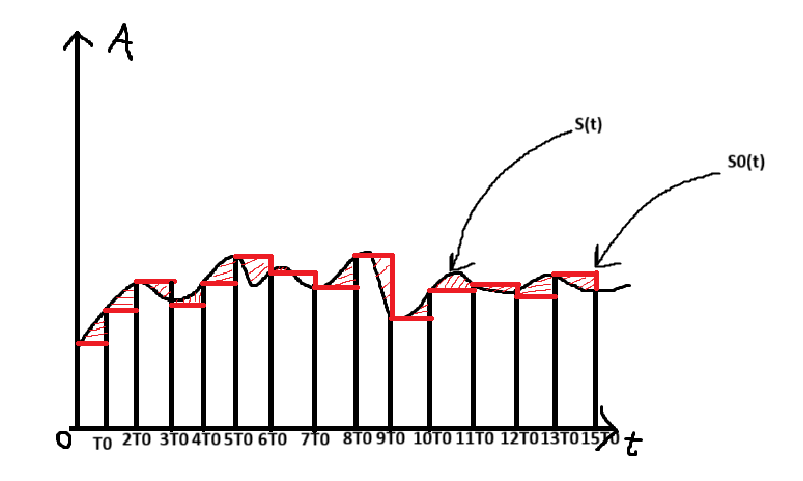
\includegraphics[width=1.0\textwidth]{aprox.png}
    \caption{Аппроксимация сигнала прямоугольными импульсами}
\end{figure}

\section*{Шаг 3}

Если просуммировать произведения выше, то получим примерное значение входной произвольной функции $S(t)$.

\[
s(t) \approx s(0) s_0(t) + s(T_0) s_0(t - T_0) + s(2T_0) s_0(t - 2T_0)
\]

Если воспользоваться свойствами LTI систем, то можем посчитать значение выходного сигнала y(t) как сумму реакций на элементарные сигналы

\[
y(t) = s(0) F[s_0(t)] + s(T_0) F[s_0(t - T_0)] + \ldots
\]

Эта аппроксимация не совсем точная (можем видеть на графике, что некотрые части произвольного сигнала теряются). Чтобы повысить
точность, нужно сделать $T_0$ максимально маленьким, т.е $T_0 \to 0$, тогда получим дельта-функцию.

\section*{Дельта функция}

Дельта-функция ($\delta(t)$) - обобщенная функция. Значение функции определяется не через аргумент, а через взаимодействие с другими
функциями.

\begin{figure}[H]
    \centering
    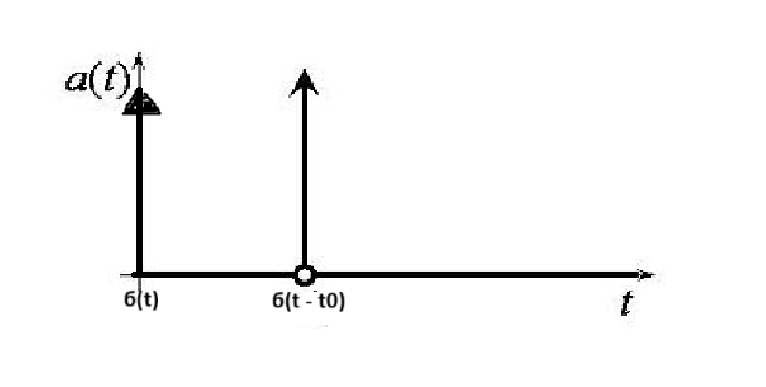
\includegraphics[width=1.0\textwidth]{delta.png}
    \caption{Дельта-функция}
\end{figure}

\subsection*{Свойства дельта-функции}

\begin{enumerate}
    \item $\delta(t) = 0$, $t \neq 0$, функция везде равна 0, кроме точки t.
    \item $\int_{-\infty}^{\infty}\delta(t)dt = 1$, площадь, занимаемая дельта-функцией, равна единице.
    \item $\int_{-\infty}^{\infty}\delta(t-t_0)dt = 1$, площадь, занимаемая дельта-функцией, равна единице и не зависит от сдвига.
    \item $\int_{-\infty}^{\infty}x(t)\delta(t-t_0)dt = \int_{-\infty}^{\infty}x(t_0)\delta(t-t_0)dt = x(t_0) * 1 = x(t_0)$, произведение функции
    и дельта-функции, сдвинутой на $t_0$, под интегралом дает значение значение функции в точке $t_0$ ($x(t_0)$) 
\end{enumerate}

\section*{Улучшение аппроксимации}

На прошлом шаге мы получили аппроксимацию для проивзольного входного сигнала. Теперь будем учитывать, что $T_0 \to 0$, поэтому 
промежутков $kT_0$ будет всё больше и больше, поэтому сумма перейдет в интеграл 

$S(t) = \int_{-\infty}^{\infty}S(\tau)\delta(t-\tau)d\tau$

\section*{Импульсная характеристика системы (импульсная реакция системы)}

При подаче $\delta(t)$ на вход LTI системы на выходе получим реакцию системы h(t)

\begin{figure}[H]
    \centering
    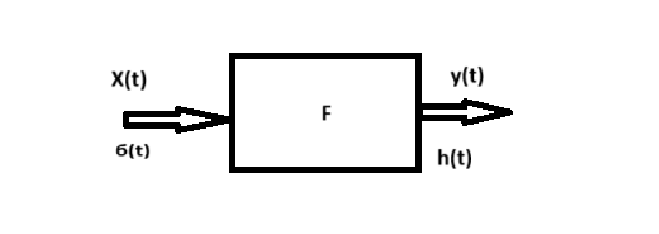
\includegraphics[width=1.0\textwidth]{imp.png}
    \caption{Реакция системы на дельта-функцию}
\end{figure}

h(t) - импульсная характеристика системы или реакция системы на дельта-функцию. \\

Таким образом выходной сигнал y(t) можно записать как

$$\boxed{y(t) =  \int_{-\infty}^{\infty}S(\tau)h(t-\tau)d\tau}$$

Формула выше - свертка, интеграл свертки. \\

Если представить входной сигнал как сумму бесконечной последовательности взвешенных и задержанных дельта-функций, то на выходе
системы получается бесконечно много взвешанных и задержанных импульсных реакций системы. Входной сигнал системы - сумма (интеграл)
по всем взвешанным и задержанным импульсным характеристикам.

\section*{Процесс свертки}

Процесс свертки сигналов выглядит следующим образом:

\begin{figure}[H]
    \centering
    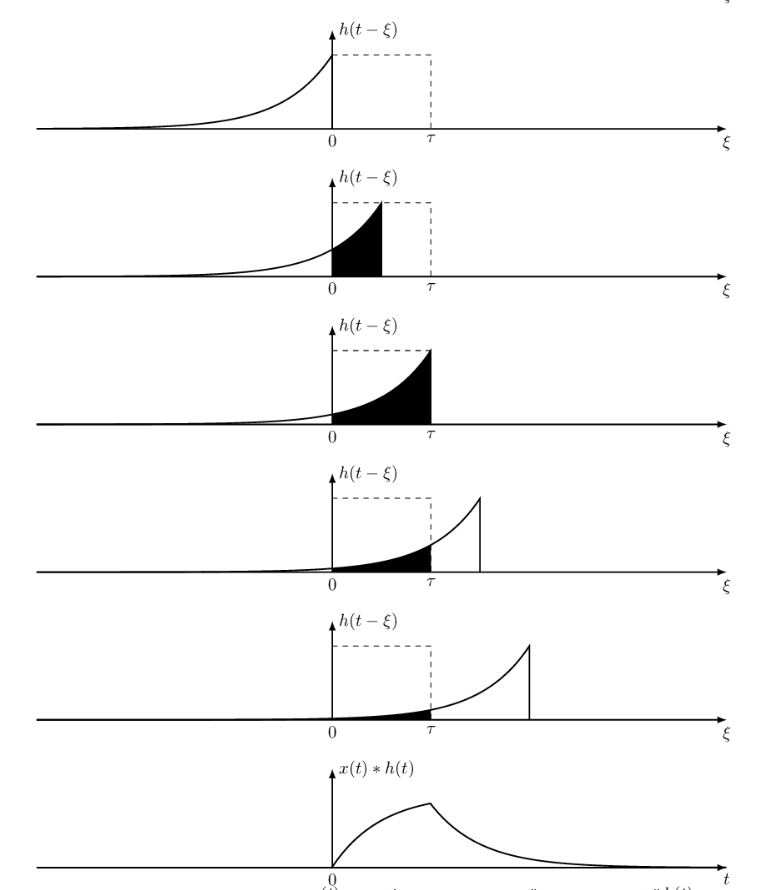
\includegraphics[width=1.0\textwidth]{svert.png}
    \caption{Визуализация процесса свертки}
\end{figure}

Здесь задан прямоугольный сигнал $S(t)$ и импульсная характеристика RC-цепи $h(-t)$. $S(t)$ остается все время неподвижным, а 
импульсная характеристика сдвигается постепенно вправо и накладывается на сигнал $S(t)$. Свертка - интеграл, значит, он будет
суммировать площадь под пересечением сигналов. \\

Если пронаблюдать за площадью, то можно заметить, что она сначала равна нулю (когда нет пересечения), потом в какой-то момент
начинает возрастать, а потом в какой-то момент начинает убывать. Эти изменения площади под пересечением графиков отражают характер
выходной сигнал  $y(t)$ - сначала он будет возрастать, потом убывать.

\section*{Промежутки свертки}

\subsection*{1) t < 0}

Возьмем любую точку t < 0 и сместим в нее график $h(-t)$ (первый график на картинке выше). 
Поскольку пересечения у графиков нет, то свертка будет равна нулю.

\subsection*{2) 0 < t < $T_0$}

$T_0$ - длительность прямоугольного сигнала\\

В этом случае t находится в прямоугольном сигнале и $h(-t)$ как-бы входит в него и образуется пересечение (2-3 график). Площадь
под пересечением графиков начинает расти. Запишем операцию свертки на этом промежутке: \\

Пусть $S(\tau) = U$, $h(t-\tau) = \frac{1}{T}e^{-\frac{t-\tau}{T}}$

$$y(t) = \int_{-\infty}^{\infty}S(\tau)h(t-\tau)d\tau = \int_{0}^{t}\frac{U}{T}e^{\frac{t-\tau}{T}}d\tau$$

Разобьем $e^{-\frac{t-\tau}{T}}$ на $e^{-\frac{t}{T}}$ и $e^{\frac{\tau}{T}}$. Заметим, что $\frac{U}{T}$ и $e^{-\frac{t}{T}}$ 
не зависисят от $\tau$, поэтому вынесем их за скобку.

$$\frac{U}{T}e^{-\frac{t}{T}}\int_{-\infty}^{\infty}e^{\frac{\tau}{T}}d\tau = \frac{U}{T}e^{-\frac{t}{T}}Te^{\frac{\tau}{T}}\bigg|_0^t = $$

$$Ue^{-\frac{t}{T}}e^{\frac{\tau}{T}}\bigg|_0^t = Ue^{-\frac{t}{T}}e^{\frac{t}{T}} - (Ue^{-\frac{t}{T}}e^{\frac{0}{T}}) = $$

$$\boxed{U[1-e^{-\frac{t}{T}}]}$$

\subsection*{3) t > $T_0$}

Если t > $T_0$, то $h(-t)$ начинается за правой границей прямоугольника (4-5 график). Площадь под пересечением графиков начинает
уменьшаться. Найдем, как будет изменяться выходной сигнал $y(t)$ на этом промежутке:

$$y(t) = \int_{0}^{T_0}\frac{U}{T}e^{\frac{t-\tau}{T}}d\tau = \frac{U}{T}e^{-\frac{t}{T}}\int_{-\infty}^{\infty}e^{\frac{\tau}{T}}d\tau = $$
$$\frac{U}{T}e^{-\frac{t}{T}}Te^{\frac{\tau}{T}}\bigg|_0^{T_0} = Ue^{-\frac{t}{T}}e^{\frac{\tau}{T}}\bigg|_0^{T_0} = $$
$$Ue^{-\frac{t}{T}}e^{\frac{T_0}{T}} - (Ue^{-\frac{t}{T}}e^{\frac{0}{T}}) = $$
$$\boxed{Ue^{-\frac{t}{T}}[e^{-\frac{T_0}{T}} - 1]}$$


\endinput